\chapter{Funktionen}

\section{Grundbegriffe}
Was ist eine Funktion? -> Definition, Notation für Beispiele und Gegenbeispiele
Urbild, Bild, Injektiv, Surjektiv, Bijektiv, Verkettung/Verknüpfung, Graph

Gleichheitsbegriff -> Wann sind zwei Funktionen "gleich"?

Was heißt es wenn sich zwei Funktionen schneiden?

Betrachten von bestimmten Arten von Funktionen in den nächsten Abschnitten. 

\begin{definition}[Definitionsbereich, Wertebereich, Bildbereich]
    Sei \(f\) eine Funktion. Dann heißt die Menge \(D\) aller Werte, für die \(f\) definiert ist, \textbf{Definitionsbereich}\index{Funktion!Definitionsbereich} von \(f\). Die Menge \(W\) aller Werte, die \(f\) über seinem Definitionsbereich annehmen kann, heißt \textbf{Wertebereich}\index{Funktion!Wertebereich} von \(f\). Jede Menge, die den Wertebereich von \(f\) enthält, heißt \textbf{Bildbereich}\index{Funktion!Bildbereich} von \(f\). 
\end{definition}
Vereinfacht gesagt besteht der Definitionsbereich aus den Werten, für die man \(f\) überhaupt betrachten möchte. Dabei muss man natürlich darauf Acht geben, dass \(f\) für einen dieser Werte auch tatsächlich einen Wert annehmen kann. Das folgende Beispiel \ref{bsp:defbereich-wertebereich-bildbereich} verdeutlicht dies. Der Wertebereich kann auch als "`minimaler"' Bildbereich von \(f\) verstanden werden. Manchmal wird auch \(\mathbb D\) für den Definitionsbereich und \(\mathbb W\) für den Wertebereich geschrieben. Diese Schreibweisen werden wir allerdings nicht weiter verfolgen. 

Damit wir später möglichst genau Eigenschaften um Funktionen herum fassen können, empfiehlt sich folgende Notation, die in der Universitäts-Mathematik Standard ist. Dabei wollen wir nicht darauf eingehen, wie Funktionen elementar definiert werden. 
\begin{definition}[Funktions-Notation]
    Sei \(f\) eine Funktion. Ist \(D\) ihr Definitionsbereich und \(B\) ihr Bildbereich, so schreiben wir 
    \begin{equation*}
        f:D \to B, \quad x \mapsto f(x)
    \end{equation*}
    und sagen "`\(f\) bildet \(x\) auf \(f(x)\) ab"'.
\end{definition}
Alternativ schreibt man statt \(x \mapsto f(x)\) auch oft direkt die Vorschrift von \(f\), das heißt zum Beispiel im Falle einer Parabel \(f(x) = x^2\) statt \(x \mapsto x^2\). Zudem gibt man den  Bildbereich meist großzügig an, da es oft zunächst nicht ganz klar ist, wie der Wertebereich zu einem speziellen Definitionsbereich genau aussieht. Um uns im Folgenden die Notation "`Sei \(f:D\to \mathbb R\) eine Funktion mit Definitionsbereich \(D\) zu sparen"' schreiben wir auch häufig "`Sei \(D\subseteq R\) und \(f:D\to\mathbb R\)"' oder wenn ein spezifisches \(D\) gegeben ist auch nur "`Sei \(f:D\to\mathbb R\) eine Funktion"'. 
\begin{example}[Definitionsbereich, Unterschied von Wertebereich und Bildbereich] \label{bsp:defbereich-wertebereich-bildbereich}
    Sei \(f(x) = \frac{1}{x}\). Diese Schreibweise ist mathematisch fahrlässig. Denn würde man die Funktion \(f\) allein durch diese Angabe definieren, so könnte man noch auf die Idee kommen, auch \(0\) in die Funktion einzusetzen. Wir wissen aber: Das Teilen durch \(0\) ist nicht definiert! Damit kann \(f\) in \(0\) gar keinen Wert annehmen. Streng genommen müssen wir also \(0\) aus den Werten ausschließen, die wir in \(f\) einsetzen können. Der Definitionsbereich von \(f\) kann also nicht die \(0\) enthalten. Für jede andere reelle Zahl ist \(f\) gibt es jedoch keine Probleme. Manchmal ist es aber trotzdem sinnvoll eine Funktion nur auf einem Teil der Werte zu betrachten, für die sie eigentlich rein mathematisch gesehen einen Wert annehmen könnte. Wir können dabei für unser spezielles \(f\) situationsabhängig jede beliebige Teilmenge \(0 \notin I\subseteq \mathbb R\) der reellen Zahlen als Definitionsbereich von \(f\) wählen, die nicht die \(0\) enthält. \par 
    Abhängig davon, über welchen Werten wir \(f\) betrachten, also welchen Definitionsbereich wir genau wählen, nimmt \(f\) verschiedene Werte an. Hier ist es also erst einmal von vorne hinein oft gar nicht genau klar, was genau der Wertebereich zu einem speziellen Definitionsbereich eigentlich ist. Deshalb gibt man in der Definition einer Funktion auch oft den Bildbereich großzügig an, also "`maximal"'. Betrachten wir in unserem Fall zum Beispiel den Definitionsbereich \(D = (0,1]\). Der dazugehörige Wertebereich ist \([1, \infty)\). Das lässt sich jetzt in unserem Fall noch relativ leicht erkennen, allerdings ist das bei komplizierteren Funktionen schon schwieriger. Deshalb schreiben wir dann \(f\) auch häufig als 
    \begin{equation*}
        f: (0,1] \to \mathbb R, \quad x \mapsto \frac{1}{x}
    \end{equation*}
    statt
    \begin{equation*}
        f: (0,1] \to [1, \infty), \quad x \mapsto \frac{1}{x}
    \end{equation*}
    Es sei zudem angemerkt, dass die Schreibweise \(f:(0,1]\to \mathbb R, f(x) = \frac{1}{x}\) ebenfalls gängig ist. 
\end{example}

Die folgende Sprechweise wird bei Extremstellen und Extrempunkten noch relevanter werden. Häufig spricht man aber auch einfach synonym von Stellen als Punkten. 
\begin{definition}[Stelle, Punkt]
    Ist \(f:D\to\mathbb R\) eine beliebige Funktion, so spricht man oft von Elementen \(x \in D\) aus dem Definitionsbereich \(D\) als \textbf{Stellen}\index{Funktion!Stelle} und von \((x,f(x))\) als zugehörigen \textbf{Punkt}\index{Funktion!Punkt}.
\end{definition}

\section{Geraden (Lineare Funktionen)}
Geraden, Sekanten, Tangenten (Nur erwähnen und auf Ableitungskapitel verweisen). 

Steigung (Noch keine genaue Vorstellung was Steigung eigentlich heißt, mehr bei Ableitungen) => Steigungsdreieck
\begin{definition}[Gerade, Konstante Funktion]
    Eine Funktion \(g:\mathbb R \to \mathbb R\) der Form 
    \begin{equation*}
        g(x) = mx + c, \quad m \in \mathbb R, x \in \mathbb R
    \end{equation*}
    heißt \textbf{Gerade}\index{Gerade}. Ist \(m=0\), so hat \(g\) die Form \(g(x) = c\) und wird dann auch \textbf{konstante Funktion} genannt. 
\end{definition}

\begin{example}
    Wir betrachten die spezielle Gerade \(g:\mathbb R \to \mathbb R, x \mapsto x\), auch \textit{Identitätsfunktion}\index{Identität, Identitätsfunktion} genannt. Dann nennen wir etwa \(1\in \mathbb R\) eine Stelle im Definitionsbereich von \(g\), während \((1,g(1)) = (1,1)\) ein Punkt ist. 
\end{example}

Eine spezielle Form von Gerade, die für die Definition und Intuition der Tangente (siehe Abschnitt Ableitung) eine entscheidende Rolle spielt, ist die Sekante.
\begin{definition}[Sekante]
    Sei \(f: D \to \mathbb R\) eine beliebige Funktion über einer Teilmenge \(D\subseteq \mathbb R\). Für zwei beliebige verschiedene Stellen $a, b \in D$ heißt die Gerade \(s\) durch die Punkte \((a,f(a))\) und \((b,f(b))\) \textbf{Sekante}\index{Sekante} von \(f\) an den Stellen \(a\) und \(b\). 
\end{definition}

\begin{wrapfigure}{r}{0.3\textwidth}
    \begin{center}
        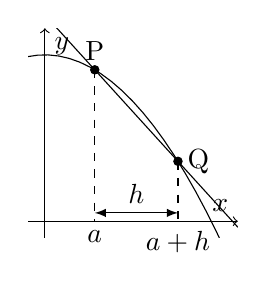
\begin{tikzpicture}[scale=1]
            \begin{axis}[
                xmin = -0.5, xmax = 5.8,
                ymin = -0.5, ymax = 5.8,
                xtick=\empty,
                ytick=\empty,
                axis x line=middle,
                axis y line=middle,
                axis line style=->,
                width = 0.35*\textwidth,
                height = 0.35*\textwidth,
                xlabel = {$x$},
                ylabel = {$y$},
                clip mode = individual,
            ]
            
            \addplot[no marks] expression[domain=-1.8:5.8]{-(1/5)*x^2+5};
            \addplot[no marks] expression[domain=-1.8:5.8]{-1.1*x+6.2};
            
            \draw[fill=black] (1.5,4.55) circle (1.5pt) node[anchor=south]{P}
            (4,1.8) circle (1.5pt) node[anchor=west]{Q};
            
            \draw[dashed] (1.5, 4.55) -- (1.5, 0) node[anchor=north]{$a$}
            (4, 1.8) -- (4, 0) node[anchor=north]{$a+h$}; 
            
            \draw[latex-latex] (1.5, 0.25) -- (4, 0.25) node[midway, anchor=south]{$h$};
                
            \end{axis}
        \end{tikzpicture}
    \end{center}

    \caption[shortlabels]{Schema\-tische Darstellung einer Sekante.}
\end{wrapfigure}

Welche Form hat eine Sekante jetzt genau? Wir fordern in unserer Definition, dass die Sekante \(s\) eine spezielle Gerade ist. Damit wissen wir, dass \(s\) allgemein die Form 
\begin{equation*}
    s(x) = mx + c
\end{equation*}
hat für ein bestimmtes \(m \in \mathbb R\) und ein bestimmtes \(c \in \mathbb R\). Nun wollen wir herausfinden, welche Form \(m\) und \(c\) genau haben müssen. Anhand unserer Definition wissen wir, dass für die Sekante \(s\) durch die Punkte \((a, f(a))\) und \((b,f(b))\) gelten muss 
\begin{align}
    \begin{split}\label{eq:sekanten-lgs}
        m a + c = s(a) &= f(a) \\
        m b + c = s(b) &= f(b)
    \end{split}
\end{align}
denn, dass die Sekante durch diese Punkte "`geht"' bedeutet nichts anderes, als dass sie an den Stellen \(\tilde x\) und \(y\) mit der Funktion \(f\) übereinstimmt. Indem wir die erste Zeile von der zweiten Zeile anziehen, erhalten wir das System
\begin{align*}
    m a + c &= f(a) \\
    mb - ma &= f(b) - f(a)
\end{align*}
Nun können wir in der zweiten Zeile auf der linken Seite \(m\) ausklammern und sofern \(b - a \neq 0\) auch durch \(b - a\) teilen. Damit erhalten wir für \(m\)
\begin{equation*}
    m = \frac{f(b) - f(a)}{b-a}
\end{equation*}
Wenn aber doch \(b - a = 0\), dann ist das für uns kein Problem. Denn dies ist nur genau dann der Fall, wenn \(b=a\). Diesen Fall haben wir aber per Definition der Sekante ausgeschlossen. Es kann jedoch natürlich trotzdem \(f(b) - f(a) = 0\) gelten und damit \(m=0\). Ein einfaches Beispiel dafür ist in Beispiel \ref{bsp:konstante-sekante} aufgeführt. Wir können also allgemein davon ausgehen, dass \(m\) die oben angegebene Form hat. Dann stellen wir die erste Zeile von \eqref{eq:sekanten-lgs} nach \(c\) um und erhalten 
\begin{align*}
    c &= f(a) - ma = f(a) - \frac{af(b) - af(a)}{b-a} = \frac{(b-a)f(a)}{b-a} - \frac{af(b) - af(a)}{b-a} \\ 
    &= \frac{bf(a) - af(a) + af(a) - af(b)}{b-a} = \frac{bf(a) - af(b)}{b-a}
\end{align*}
Damit haben wir insgesamt gezeigt
\begin{proposition}[Form der Sekante]\label{prop:form-der-sekante}
    Sei \(s\) die Sekante einer Funktion \(f\) an den Stellen \(a\) und \(b\). Dann gilt 
    \begin{equation*}
        s(x) = \frac{f(b) - f(a)}{b-a}\cdot x + \frac{bf(a) - af(b)}{b-a}
    \end{equation*}
\end{proposition}

\begin{example}[Konstante Sekante]\label{bsp:konstante-sekante}
    Sei \(f(x)=x^2\) die Parabel. Dann gilt für die Stellen \(-1\) und \(1\), dass \(f(-1) = 1 = f(1)\). Nach Proposition \ref{prop:form-der-sekante} gilt dann für die Sekante \(s\) von \(f\) an den Stellen \(-1\) und \(1\) 
    \begin{equation*}
        s(x) = 0 \cdot x + \frac{1\cdot f(-1)-(-1)\cdot f(1)}{1 - (-1)} = 2
    \end{equation*}
\end{example}
Aus unserer Herleitung von Proposition \ref{prop:form-der-sekante} über die Form einer Sekante können wir sogar allgemein ablesen, wie wir die Geradengleichung einer beliebigen Gerade durch zwei beliebige Punkte aufstellen können. 

\begin{problem}[Bestimmen einer Geradengleichung]
    Existiert eine Gerade \(g: \mathbb R\to\mathbb R\), welche durch gegebene Punkte geht? Und wenn ja, wie erhält man ihre Form? Um diese Fragen vollständig zu beantworten, betrachten wir drei Fälle: 
    \begin{enumerate}
        \item Ein Punkt \((a,b)\) ist gegeben. In diesem Fall finden wir \normal{beliebig viele} Geraden, die durch diesen Punkt gehen. \par
        \begin{normalfont}
            Dies ist anschaulich klar. Rein mathematisch gesehen können wir uns folgendes überlegen: Sei \((a,b)\) ein vorgegebener Punkt und \(g:\mathbb R\to\mathbb R\) eine allgemeine Gerade, d.h. \(g(x) = mx+c\) für ein \(m\in \mathbb R\) und \(c\in \mathbb R\). Es muss dann gelten 
            \begin{equation*}
                ma + c = g(a) = b
            \end{equation*}
            Wir haben also eine Gleichung mit zwei Unbekannten \(m,c\). Lösen wir diese nach \(c\) auf, so ist \(c = b - ma\). Damit sind alle Geraden der Form \(g(x) = mx + (b-ma)\) für beliebiges \(m \in \mathbb R\) Geraden, auf welchen der Punkt \((a,b)\) liegt. 
        \end{normalfont}
        
        \item Zwei Punkte \((a_1,b_1)\) und \((a_2, b_2)\) sind gegeben. In diesem Fall finden wir \normal{genau eine} Gerade, die durch diese beiden Punkte geht. \par
        \begin{normalfont}
            Hier können wir exakt so vorgehen wir beim Bestimmen der allgemeinen Form der Sekante. Proposition \ref{prop:form-der-sekante} liefert dann also für die die gesuchte Gerade \(g:\mathbb R\to \mathbb R\) als Sekante von der Identitätsfunktion \(f(x) = x\) durch die Punkte \((a_1 , b_1)\) und \((a_2, b_2)\) die Form
            \begin{equation*}
                g(x) = \frac{b_2 - b_1}{a_2 - a_1}x + \frac{a_2b_1 - a_1b_2}{a_2 - a_1}
            \end{equation*}
        \end{normalfont}
        
        \item Mehr als zwei Punkte \((a_1, b_1), (a_2, b_2), \dots, (a_n, b_n)\) sind gegeben. In diesem Fall muss nicht zwingend eine Gerade existieren, auf der alle gegebenen Punkte liegen. \par
        \begin{normalfont}
            
        \end{normalfont}
    \end{enumerate}
\end{problem}

\section{Ganzrationale Funktionen (Polynome)}

Anwendung: Ordnung eines Polynoms aus einem logarithmischen Plot bestimmen. 

Exkurs: Algebraische Relevanz => Polynomringe, Polynomräume, Alles sind Polynome (Taylor-Entwicklung!), Numerische Interpolation

\begin{definition}[Ganzrationale Funktion/Polynomfunktion]
    
\end{definition}

\begin{definition}[Parabel, Kubische Funktion]
    
\end{definition}

Linearfaktoren: Zerlegung in Nullstellen, Fundamentalsatz der Algebra, Grad eines Polynoms und maximale Anzahl an Nullstellen.

\begin{theorem}[Linearfaktorzerlegung]
    
\end{theorem}

\begin{theorem}[Maximale Anzahl an Nullstellen]
    
\end{theorem}

\begin{theorem}[Fundamentalsatz der Algebra]
    
\end{theorem}

Nullstellen bestimmen: abc-/Mitternachtsformel, pq-Formel, Satz von Vieta (Verweis auf Merksongs von Dorfuchs) + Beweise!

\begin{theorem}[abc-/Mitternachtsformel]
    
\end{theorem}

\begin{theorem}[pq-Formel]
    
\end{theorem}

\begin{theorem}[Satz von Vieta]
    
\end{theorem}

\begin{theorem}[Polynomdivision]
    
\end{theorem}


\section{Gebrochenrationale Funktionen}

\begin{definition}[Gebrochenrationale Funktion]
    
\end{definition}

Grundbegriffe: Definitionslücken und Polstellen + Asymptoten (Verweis auf später)

\begin{definition}[(Hebbare) Definitionslücke]
    
\end{definition}

\begin{definition}[Polstelle]
    
\end{definition}

\section{Exponentialfunktionen und Logarithmen}
Allgemeine Exponentialfunktionen und deren Umkehrfunktionen!
=> Rechnen mit Logarithmen: Gleichungen mit unbekannten im Exponenten lösen (Oft benötigt für Wahrscheinlichkeiten => Verweis auf entsprechende Probleme). 

Logarithmusgesetze

Was bedeutet es, mit einer irrationalen Zahl zu potenzieren, z.b. \(2^\pi\)? => Wie ist das rigoros definiert? => Mehr später im Abschnitt zur eulerschen Zahl \(e\)

Herleitung durch gleichbleibende Ableitung (Vorgreifen). 

In Beispielen in Ableitungskapitel (Oder Proposition), die Ableitungen bestimmen. 

\section{Trigonometrische Funktionen}

\subsection{Sinus, Kosinus und Tangens}
Historische Definition von sin, cos, tan am Einheitskreis: Hypotenuse, Ankathete, Gegenkathete => Hint auf späteren Exkurs mit der Exponentialfunktion und den komplexen Zahlen

\begin{definition}[Historische Definition von Sinus und Cosinus]
    
\end{definition}

Exkurs: Sinus, Cosinus, Tangens in Reihendarstellung

\begin{definition}[Analytische Definition von Sinus und Cosinus]
    
\end{definition}

Eigenschaften von sin und cos: Nullstellen, Extremstellen, Ableitung, Stammfunktion, Umkehrfunktion (arcsin, arccos)

Die Kreiszahl \(\pi\): Historische Definition: Verhältnis von Kreisumfang zu irgendwas anderem VS. analytische Definition als kleinste Nullstelle des Cosinus. 

Interessantes Beispiel: Anwendung der irrationalität von \(\pi\). 

Satz: Additionstheoreme (Verweis auf Dorfuchs-Video für Merksong)
\begin{theorem}[Additionstheoreme]
    
\end{theorem}

\begin{corollary}[Doppelwinkelformeln]
    
\end{corollary}

Untersuchung von periodischen Funktionen: Wie kann man die Periode aus einem veränderten sin, cos ablesen? Wie verändert sich die Periode bei Streckungen/Stauchungen?

Wie berechnet der Taschenrechner Sinus und Kosinus => Taylor-Entwicklung! (Fehlerabschätzung)

\subsection{Bogenmaß und Gradmaß}


\section{Funktionsscharen}
Typische Aufgaben: Bestimme Gemeinsamkeiten usw. 

Bestimmen von Ortskurven